\chapter{Грани, их размерность}
\label{cha:11}

\epigraph{
	\textit{Но какая же разница и в средствах и в размерах!}}
{-- Добролюбов Н.А.}

\begin{propose}\label{cha:11/propose:1}
	Пусть полиэдр P задается системой аффинных неравенств (5), а грань $\Gamma_A$, $A \in P$, задается уравнениями $f_1 = \dots = f_r = 0$. Если ранг линейных частей системы функций $f_1, \dots, f_r$ равен k, то $dim \Gamma_A = dim P − k$.
\end{propose}
\begin{Proof}
	Можно считать, что все пространство является минимальной плоскостью, содержащей P. Предположим, что ранг линейных частей системы $f_1, \dots, f_r$ равен k, и $\Pi$ – плоскость, задаваемая системой уравнений $f_1 = \dots = f_r = 0$. Пусть $U \subset \mathbb{A}^n$ – множество всех таких точек $B \in \mathbb{A}^n$, что $f_{r+1}(B) > 0, \dots, f_m(B) > 0$. Тогда $U \cap \Pi \subset \Gamma_A$, причем
	$$dim \Gamma_A = dim <U \cap \Pi> = dim \Pi = dim P - k$$
\end{Proof}

\begin{theorem}[]\label{cha:11/the:1}
	Пусть полиэдр P задан системой аффинных неравенств (5), и $f_1, \dots, f_r$ не равны тождественно нулю на P, но $f_{r+1} |_P = \dots = f_m |_P = 0$. Обозначим через $\Pi_i$ гиперплоскость, задаваемую уравнением $f_i = 0$, где $1 \le i \le r$. Тогда $\Pi_i \cap P$ является гранью размерности $dim P − 1$ в P для некоторого i.
\end{theorem}
\begin{Proof}
	Без ограничения общности можно считать, что гиперплоскости $\Pi_1, \dots, \Pi_r$ различны. Пусть A – внутренняя точка в P. По предложению \ref{cha:10/propose:2} $f_1(A) > 0, \dots, f_r(A) > 0$. Переходя к плоскости, порожденной P, можно считать, что эта плоскость совпадает с $\mathbb{A}^n$ и $r = m$. Предположим, что $f_i(x) = a_i + \underset{j=1}{\overset{n}{\sum}} a_{ij} x_j$. Обозначим через $B_i$ проекцию A на $\Pi_i$. Как известно:
	$$||\overline{AB}|| = \frac{|f_i (A)|}{\sqrt{a_{i1}^2 + \dots + a_{in}^2}}\eqno(26)$$
	Пусть U – открытый шар в $\mathbb{A}^n$ с центром в точке A, целиком содержащийся в P. По (26) все точки $X \in \mathbb{A}^n$, равноудаленные от различных гиперплоскостей $\Pi_i, \Pi_j$ при $i \not = j$ образуют пару гиперплоскостей, задаваемых уравнениями:
	$$\frac{|f_i (X)|}{\sqrt{a_{i1}^2 + \dots + a_{in}^2}} = \frac{|f_j (X)|}{\sqrt{a_{j1}^2 + \dots + a_{jn}^2}}$$
	Объединение всех этих гиперплоскостей по всем парам $1 \le i \not = j \le n$ не покрывает все U. Следовательно, в U существует такая внутренняя точка B, расстояния от которой до $\Pi_1, \dots, \Pi_r$ различны. Без ограничения общности можно считать, что $||\overline{BB_1}|| < ||\overline{BB_2}|| < \dots < ||\overline{BB_r}||$.

	\begin{lemma}\label{cha:11/lemma:1}
		Точка $B_1$ принадлежит P.
	\end{lemma}
	\begin{Proof}
		Пусть $B_1 \not \in P$. Тогда существует такое $i = 2, \dots, n$, что $f_i(B_1) < 0$. Пусть, например, $f_2(B_1) < 0$.

		\begin{center}
			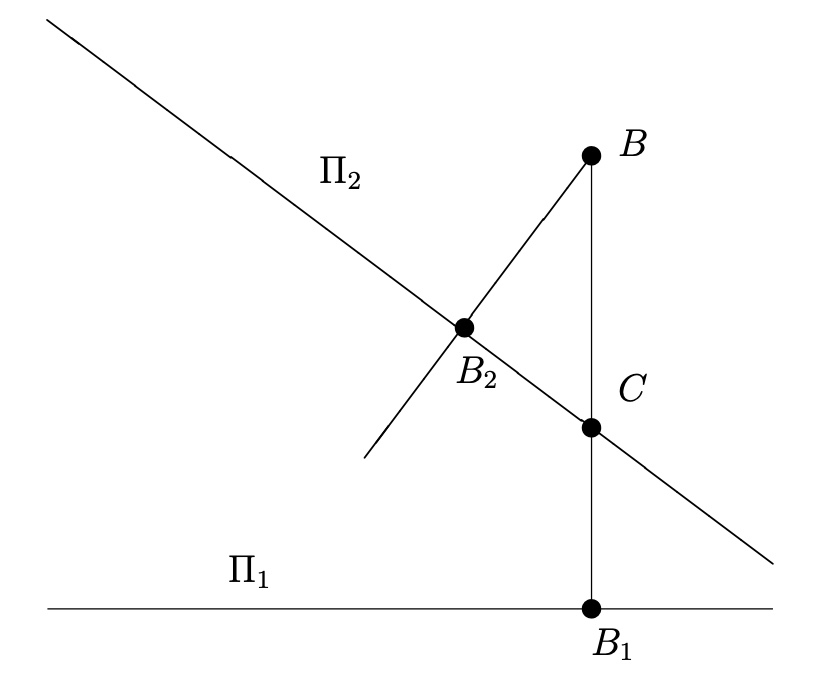
\includegraphics[width=\textwidth]{11_1}
		\end{center}

		Так как $f_2(B) > 0$, то на интервале $(B,B_1)$ найдется такая точка C, что $f_2(C) = 0$. В этом случае $C \in \Pi_2$, причем $||\overline{BC}|| \ge || \overline{BB_2}||$. Отсюда $||\overline{BB_1}|| > ||\overline{BC}|| \ge || \overline{BB_2}||$, что противоречит предположению.
	\end{Proof}

	Завершим доказательство теоремы. Заметим, что $B_1 \not \in \Pi_i$ при $i \ge 2$. Действительно, если $B_1 \in \Pi_i$ и $i \ge 2$, то $||\overline{BB_2}|| \le ||\overline{BB_1}||$, что неверно. Таким образом, $f_2 (B_1) > 0, \dots, f_n (B_1) > 0$, т.е. $\Gamma_{B_1} = \Pi_1 \cap P$. При этом:
	$$dim \Gamma_{B_1} = dim \Pi_1 = n-1 = dim P - 1$$
\end{Proof}
